\documentclass[../Proposal.tex]{subfiles}
 
\begin{document}
	\section{Dataset}
	\textit{Dataset} yang digunakan pada tugas akhir ini diambil di \textit{web} resmi PAN\cite{pan-task-2014}. Gambar \ref{fig:Dataset} menunjukan hierarki dari \textit{dataset} yang digunakan.
	
	\newpage
	
	\begin{figure}[h!]
		
		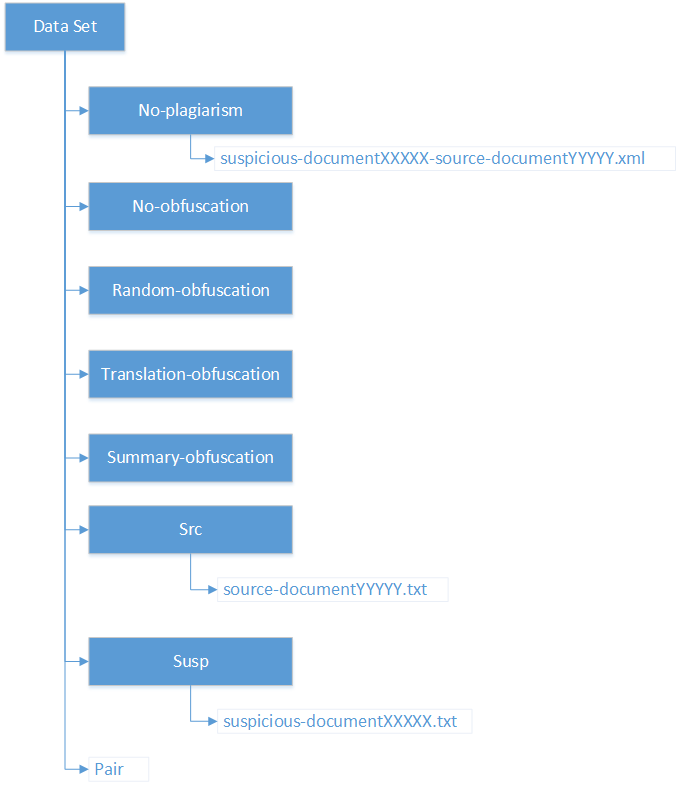
\includegraphics[width=340pt]{hierarkids}
		\caption[Dataset]{Dataset}
		\label{fig:Dataset}
	\end{figure}
	
	\textit{Dataset} diatas mempunyai bagian-bagian umum sebagai berikut : 
	\begin{enumerate}
		\item \textbf{Susp}\\
		Kumpulan dokumen yang terindikasi plagiat melalui proses \textit{Source Retrieval}.
		\item \textbf{Src}\\
		Merupakan dokumen sumber di plagiat oleh dokumen Susp melalui proses \textit{Source Retrieval}.
		\item \textbf{Pair}\\
		Merupakan informasi pasangan dokumen yang terindikasi, formatnya adalah \textit{suspicious-documentXXXXX.txt source-documentYYYYY.txt}. Dimana \textit{suspicious-documentXXXXX.txt} merujuk pada dokumen yang ada di Susp, dan \textit{source-documentYYYYY.txt} merujuk pada dokumen yang ada di Src.
		\item \textbf{\textit{No-Plagiarism, No-Obfuscation, Random-Obfuscation, -Obfuscation, Summary-Obfuscation}}\\
		Bagian ini merupakan kelas hasil klasifikasi tindak plagiat dari file Pair.
		\begin{enumerate}
			\item \textit{\textbf{No-Plagiarism}} : Tidak terdeketsi tindak plagiat.
			\item \textit{\textbf{No-Obfuscation}} : Tindak plagiat berupa \textit{copy-paste}.
			\item \textit{\textbf{Random-Obfuscation}} : Tindak plagiat berupa menghilang / menambahkan kata pada kalimat yang digunakan.
			\item \textit{\textbf{Translation-Obfuscation}} : Tindak plagiat berupa menerjemahkan kata.
			\item \textit{\textbf{Summary-Obfuscation}} : Tindak plagiat berupa merangkum suatu kalimat/paragraf.
		\end{enumerate}
	\end{enumerate}
	
	Sebagai contoh, pada file \textit{pairs} terdapat informasi sebagai berikut : 
	
	\begin{center}
		\centering
		\begin{equation}
		suspicious-document00005.txt source-document01496.txt
		\end{equation}
	\end{center}
	
	\noindent Berarti, menurut proses proses \textit{Source Retrieval} terdapat indikasi plagiat dari dokumen \textit{suspicious-document00005.txt} bersumber dari dokumen \textit{source-document01496.txt}. Dan menurut data yang ada, tindak plagiat pada dokumen tadi termasuk ke dalam \textit{No-Obfuscation}, dimana tindak plagiat yang dilakukan berupa \textit{copy-paste}. Dan setelah diteliti, tindak plagiat terbukti dikarenakan pada kedua dokumen terdapat kalimat yang sama. \\
	
	\noindent Berikut merupakan potongan dokumen \textit{suspicious-document00005.txt} : \\
	
	\textit{.....WAYS TO SEND YOUR DOCUMENTATION Fax to 304-724-0909 Scan and email to DSA@apus.edu Mail to APUS ATTN : Disability Accomodations 10110 Battleview Parkway Suite 114 Manassas, VA 20109 \hl{x ED502 * required berfore student may register for courses Prepare a short essay of approximately 300 words (one page) describing why you are interested in this particular degree program. Your sample should preferably be written in Word and double-spaced. The Education degree coordinator will use your writing sample to assess your written communications skills.\\ * Writing Sample Two character references are required from people who can attest to your moral and ethical character. Example of such people include supervisors, religious leaders, military commanders, school officials, or others who know you well and can provide credible information about you.} He served at the Pentagon as par of Joint Staff in support of Noble Eagle and Enduring Freedom.....} \\
	
	\noindent Berikut merupakan potongan dokumen \textit{source-document01496.txt} : \\
	
	\textit{\hl{x ED502 * required berfore student may register for courses Prepare a short essay of approximately 300 words (one page) describing why you are interested in this particular degree program. Your sample should preferably be written in Word and double-spaced. The Education degree coordinator will use your writing sample to assess your written communications skills.\\ * Writing Sample Two character references are required from people who can attest to your moral and ethical character. Example of such people include supervisors, religious leaders, military commanders, school officials, or others who know you well and can provide credible information about you.} Forms will be provided to you by your admissions representative. Once forms are completed and signed by the references, send them to APUS following the document submission instructions below.....} \\
	
	Bagian yang di \textit{highlight} merupakan bagian yang berhasil diindikasi adanya tindak plagiat.
\end{document}